\documentclass[12pt,oneside]{book}

\usepackage[utf8]{inputenc}
\usepackage[T1]{fontenc}
\usepackage{lmodern}
\usepackage[a4paper,margin=1in]{geometry}
\usepackage{setspace}
\usepackage{graphicx}
\usepackage{booktabs}
\usepackage{tabularx}
\usepackage{longtable}
\usepackage{array}
\usepackage{enumitem}
\usepackage{xcolor}
\usepackage{tikz}
\usepackage{listings}
\usepackage[numbers,sort&compress]{natbib}
\usepackage[hidelinks]{hyperref}
\usepackage[nameinlink,noabbrev]{cleveref}

\usetikzlibrary{arrows.meta,positioning,fit,shapes.geometric}
\graphicspath{{figures/}{../screenshots/webgui/}}
\onehalfspacing

\setlist[itemize]{leftmargin=1.4em}
\setlist[enumerate]{leftmargin=1.6em}

\definecolor{codegray}{RGB}{245,245,245}
\lstset{
  basicstyle=\ttfamily\small,
  backgroundcolor=\color{codegray},
  frame=single,
  breaklines=true,
  columns=fullflexible
}

\newcommand{\systemname}{CrossMedia-PID}
\newcommand{\moduleA}{Visual Extractor}
\newcommand{\moduleB}{VLM Feature Extractor}
\newcommand{\moduleC}{Hybrid Vectorizer}
\newcommand{\moduleD}{Identity Matcher}


\newcommand{\dissertationtitle}{CrossMedia-PID: Vision--Language Attribute Representation for Cross-Media Person Identification}
\newcommand{\studentname}{[Your Name]}
\newcommand{\studentid}{[Your Student ID]}
\newcommand{\supervisor}{[Supervisor Name]}
\newcommand{\department}{[Department Name]}
\newcommand{\institution}{The University of Hong Kong}
\newcommand{\submissiondate}{\today}

\begin{document}

\frontmatter
\begin{titlepage}
  \centering
  \vspace*{2cm}
  {\Large \institution\par}
  \vspace{1.5cm}
  {\huge\bfseries \dissertationtitle\par}
  \vspace{1cm}
  {\Large A Paper-Based Dissertation Draft\par}
  \vspace{2cm}
  \begin{tabular}{rl}
    Student: & \studentname \\
    Student ID: & \studentid \\
    Supervisor: & \supervisor \\
    Department: & \department \\
    Date: & \submissiondate \\
  \end{tabular}
  \vfill
  {\large Draft for Overleaf migration and supervisor discussion\par}
\end{titlepage}

\chapter*{Abstract}
\addcontentsline{toc}{chapter}{Abstract}

Person identification across images, videos, and textual descriptions remains difficult when only partial, low-resolution, or viewpoint-dependent evidence is available. Conventional person re-identification systems typically learn visual embeddings from camera-to-camera image pairs, while practical investigative workflows often require a more flexible form of matching: an operator may start from a still image, a short surveillance clip, or a natural-language description of clothing and appearance. This dissertation develops \systemname, a modular cross-media person identification system that uses vision--language models to extract structured person attributes and combines them with dense semantic embeddings for identity matching.

The dissertation is written as a multi-paper thesis. Paper I introduces the core \systemname\ architecture: a YOLO-based visual extractor, a VLM-based attribute extractor, a hybrid dense--sparse vectorizer, and an identity matcher backed by a persistent vector database. Paper II presents a video-centric testing and dataset creation interface that converts tracked person trajectories into reusable crop datasets with manifests and positive/negative matching pairs. Paper III, currently framed as a manuscript-in-preparation, formalizes the dynamic attribute registry and outlines an evaluation protocol for extending \systemname\ toward text-to-person retrieval and larger-scale cross-media benchmarks.

The current prototype demonstrates the feasibility of combining open-domain visual attributes with vector retrieval. Preliminary experiments show stable same-person matching in controlled image-pair and video-frame scenarios, while also exposing limitations related to VLM variability, small-scale evaluation, and dependence on attribute visibility. The dissertation argues that attribute-grounded hybrid representations are a promising bridge between black-box visual embeddings and interpretable cross-media search, especially when systems must support human inspection, dataset construction, and incremental experimentation.

\vspace{1em}
\noindent\textbf{Keywords:} person identification; person re-identification; vision--language models; attribute extraction; vector database; video analytics; cross-media retrieval.

\chapter*{Acknowledgements}
\addcontentsline{toc}{chapter}{Acknowledgements}

I am grateful to my supervisor, department, and peers for their guidance and feedback throughout the development of this project. I also thank the open-source communities whose tools made the implementation and experimentation possible.

This acknowledgement section should be personalized before final submission.


\tableofcontents
\listoffigures
\listoftables

\mainmatter

\part{Integrative Dissertation Chapters}
\chapter{Introduction}
\label{ch:introduction}

\section{Research Motivation}

Person identification is a recurring requirement in security, surveillance, multimedia search, and human-centred video analytics. A practical investigator may need to answer questions such as whether a person appearing in one video segment is the same person shown in another camera view, whether a still photograph corresponds to a person in a surveillance clip, or whether a natural-language description such as ``a young man wearing a black T-shirt with a white logo'' can retrieve candidate appearances from a video archive. These use cases go beyond conventional closed-set classification because the system must compare visual evidence across different media, resolutions, viewpoints, and temporal contexts.

Traditional person re-identification (Re-ID) research has made substantial progress by learning discriminative visual embeddings for matching images of pedestrians across cameras \citep{zheng2016person,ye2021deep}. However, many Re-ID systems remain difficult to inspect: they return similarity scores but provide limited explanation of which visible traits supported the match. At the same time, modern vision--language models (VLMs) have become capable of producing rich open-domain descriptions of people, clothing, and accessories \citep{radford2021learning,bai2023qwenvl}. This dissertation explores whether VLM-derived attributes can provide a useful bridge between interpretable human descriptions and vector-based retrieval.

\systemname\ is developed as a prototype for this problem. Instead of treating a person crop only as a visual embedding, the system first detects the person, extracts structured visual attributes using a VLM, converts the attributes into both dense semantic vectors and sparse attribute indicators, and then performs identity matching using a weighted hybrid similarity function. The system is designed as an experimental research artifact: it includes a command-line interface, a Streamlit graphical interface, a persistent vector database, and a test dataset creation workflow for extracting person crops from videos.

\section{Problem Statement}

This dissertation studies the following research problem:

\begin{quote}
How can a modular vision--language pipeline represent and match person identities across images and video frames while preserving enough attribute-level structure for inspection, dataset construction, and future text-based retrieval?
\end{quote}

The problem contains three technical tensions. First, visual appearance is high-dimensional and viewpoint-sensitive, so purely symbolic attributes may be too brittle. Second, learned dense embeddings can be effective but often opaque. Third, real-world evaluation requires repeatable datasets and labelled matching pairs, yet early-stage prototypes often lack a convenient mechanism for constructing such datasets from video. The current work responds to these tensions through a hybrid dense--sparse representation and a GUI-supported dataset creation pipeline.

\section{Research Objectives}

The project has five objectives:

\begin{enumerate}
  \item Develop a modular person identification pipeline that processes images and video frames using separate detection, feature extraction, vectorization, and matching modules.
  \item Use a vision--language model to extract structured, interpretable person attributes such as clothing colour, clothing type, accessories, hair style, and distinctive patterns.
  \item Combine dense semantic embeddings with sparse attribute vectors to support both flexible retrieval and inspectable matching evidence.
  \item Implement a persistent vector storage and retrieval layer for incremental identity matching.
  \item Build a GUI-assisted testing workflow that can track persons in video, select trajectories, export reusable test datasets, and run same-person matching checks.
\end{enumerate}

\section{Current Contributions}

At the current stage, the dissertation makes the following contributions.

\begin{itemize}
  \item \textbf{A modular prototype architecture.} \systemname\ separates visual extraction, VLM feature extraction, vectorization, matching, configuration, and interface layers. This makes the system easier to test and extend.
  \item \textbf{A hybrid attribute representation.} The system converts VLM attributes into dense text embeddings and sparse registry-based vectors, then combines cosine similarity and sparse overlap in a configurable matcher.
  \item \textbf{A video-to-testset GUI workflow.} The Streamlit interface supports video upload, person trajectory extraction, manual track selection, crop export, manifest generation, positive/negative pair generation, and ZIP download.
  \item \textbf{A reproducible software artifact.} The repository now contains an Overleaf-ready dissertation draft, a Python package structure, configuration templates without embedded secrets, and lightweight automated tests for dataset export.
\end{itemize}

\section{Dissertation Organization}

This dissertation is organized as a paper-based thesis. \Cref{ch:integrative-methodology} provides the unifying system methodology. \Cref{paper:hybrid-vlm-pid} is the first manuscript and focuses on the core hybrid representation and identity matching architecture. \Cref{paper:video-testset-gui} is the second manuscript and focuses on video-driven test dataset creation and GUI-supported evaluation. \Cref{paper:attribute-registry-protocol} is a third manuscript-in-preparation that formalizes the dynamic attribute registry and outlines the next-stage evaluation protocol. The final chapters synthesize the results, limitations, and future research directions.

\chapter{Literature Review}
\label{ch:literature-review}

\section{Person Re-Identification}

Person re-identification (Re-ID) studies the problem of retrieving images of the same pedestrian identity across cameras, viewpoints, and times. Early benchmarks such as CUHK03 and Market-1501 established the image-based retrieval setting and evaluation metrics that remain influential in later work \citep{li2014deepreid,zheng2015scalable}. Deep Re-ID systems generally learn an embedding space in which same-identity samples are close and different-identity samples are distant. Modern surveys describe the evolution from hand-crafted descriptors to convolutional, part-based, transformer-based, and unsupervised approaches \citep{zheng2016person,ye2021deep}.

Although Re-ID methods are highly relevant to this dissertation, the \systemname\ objective is slightly different. Standard Re-ID usually assumes that query and gallery are both person images and that the main goal is ranking images. In contrast, this project is interested in cross-media workflows in which the query may be a video frame, a still image, or a textual description. It also prioritizes inspectable attributes because the user may want to understand why two appearances were matched.

\section{Video-Based Person Identification}

Video-based Re-ID extends image Re-ID by using temporal evidence from tracklets. Datasets such as MARS and methods using recurrent or temporal pooling architectures show that temporal information can help when single frames are noisy \citep{zheng2016mars,mcLaughlin2016recurrent}. However, video also introduces practical difficulties: tracks may fragment, bounding boxes may drift, and a person may be visible only at low resolution or under occlusion. The current \systemname\ GUI therefore treats video as a source for controlled dataset construction rather than assuming that fully automatic tracking is already solved.

\section{Attribute-Based Person Description}

Person attributes provide a semantic layer between low-level visual features and human language. Datasets and methods for pedestrian attribute recognition, such as PETA and attribute-driven Re-ID, show that clothing, accessories, and body-related cues can support retrieval and explanation \citep{deng2014pedestrian,su2016deep}. Attribute methods are attractive for dissertation work because they make matching evidence more interpretable: if a match succeeds because both crops are described as wearing black upper clothing and white shoes, that evidence can be inspected by a researcher.

The limitation is that attributes are not always stable. A backpack may be occluded in one view, a logo may be too small to read, and colour descriptions may vary under lighting changes. This motivates a hybrid representation rather than an attribute-only method.

\section{Text-Based Person Search}

Text-based person search investigates retrieval of pedestrian images from natural-language descriptions. The CUHK-PEDES task introduced by \citet{li2017personsearch} is especially relevant because it directly connects language descriptions with person images. Later work has explored cross-modal alignment, transformer encoders, and vision-language pretraining for this task. Text-based person search informs the future direction of \systemname: if VLM-extracted attributes and user-written descriptions can be mapped into a shared representation, the same database could support image-to-image, video-to-image, and text-to-person retrieval.

\section{Vision--Language Models}

Vision--language models learn or prompt joint representations of images and language. CLIP demonstrated that large-scale image--text contrastive pretraining can produce transferable visual representations \citep{radford2021learning}. Qwen-VL and later Qwen2.5-VL models extend this direction toward richer visual understanding and instruction-following behaviour \citep{bai2023qwenvl,bai2025qwenvl}. For \systemname, the key property of VLMs is not only their embedding ability but also their capacity to produce structured natural-language or JSON-like descriptions of a person crop.

Recent Re-ID work has also begun to exploit vision--language models. CLIP-ReID adapts CLIP-style pretraining to image re-identification, suggesting that language-supervised visual representations can improve Re-ID transfer \citep{li2023clipreid}. This dissertation differs by using VLMs as an explicit attribute extraction module rather than only as a pretrained visual backbone.

\section{Vector Retrieval and Hybrid Representations}

Vector databases make it convenient to store embeddings and query nearest neighbours as a system grows. ChromaDB is used in this project as a lightweight persistent embedding store \citep{chroma2024}. However, dense vector retrieval alone can be opaque. Sparse representations, by contrast, can expose which attribute dimensions overlap, but they may be brittle when attributes are missing or phrased differently. The hybrid design in \systemname\ therefore follows a pragmatic principle: use dense vectors for semantic flexibility and sparse vectors for attribute-level structure.

\section{Research Gap}

The reviewed literature suggests three gaps that this dissertation addresses. First, many Re-ID systems are optimized for benchmark ranking but not for iterative cross-media investigation. Second, text-based person search connects language and images but often assumes curated text descriptions rather than VLM-extracted attributes from arbitrary crops. Third, early-stage prototypes frequently lack a reproducible pathway from raw video to labelled evaluation pairs. \systemname\ addresses these gaps through a modular VLM-assisted matching system and a GUI-supported testset creation workflow.

\chapter{Integrative Methodology}
\label{ch:integrative-methodology}

\section{System Overview}

\systemname\ is designed as a modular pipeline rather than a monolithic model. The central assumption is that cross-media person identification benefits from decomposing the task into interpretable stages: detect the person, describe the person, represent the description, retrieve candidates, and then decide whether the person should be treated as a known or new identity. \Cref{fig:system-architecture} summarizes the current pipeline.

\begin{figure}[htbp]
  \centering
  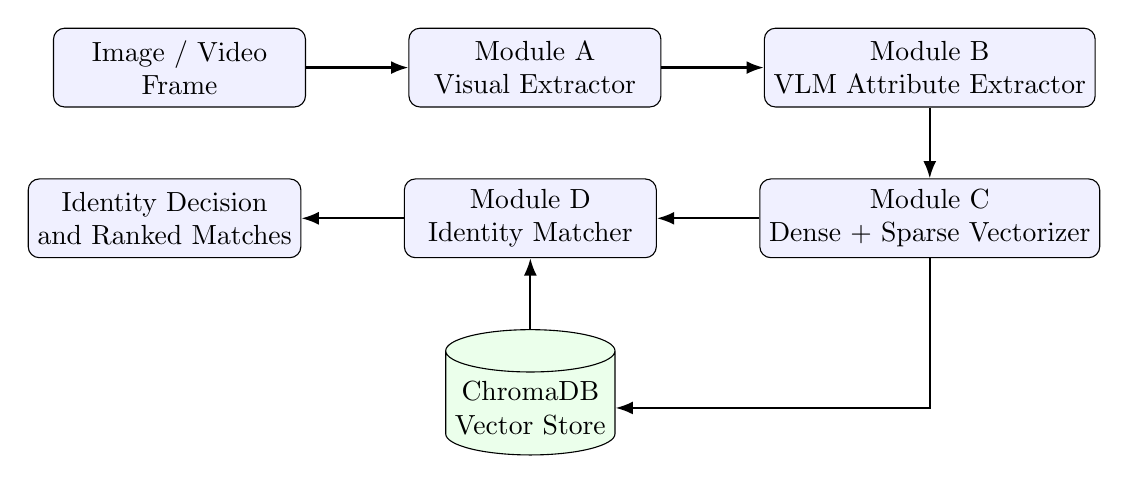
\begin{tikzpicture}[
  node distance=0.9cm and 1.3cm,
  box/.style={draw, rounded corners, align=center, minimum width=3.2cm, minimum height=1cm, fill=blue!6},
  store/.style={draw, cylinder, shape border rotate=90, aspect=0.25, align=center, minimum height=1.2cm, minimum width=1.6cm, fill=green!8},
  arrow/.style={-{Latex[length=2.2mm]}, thick}
]
\node[box] (input) {Image / Video\\Frame};
\node[box, right=of input] (detector) {Module A\\Visual Extractor};
\node[box, right=of detector] (vlm) {Module B\\VLM Attribute Extractor};
\node[box, below=of vlm] (vectorizer) {Module C\\Dense + Sparse Vectorizer};
\node[box, left=of vectorizer] (matcher) {Module D\\Identity Matcher};
\node[store, below=of matcher] (db) {ChromaDB\\Vector Store};
\node[box, left=of matcher] (output) {Identity Decision\\and Ranked Matches};

\draw[arrow] (input) -- (detector);
\draw[arrow] (detector) -- (vlm);
\draw[arrow] (vlm) -- (vectorizer);
\draw[arrow] (vectorizer) -- (matcher);
\draw[arrow] (matcher) -- (output);
\draw[arrow] (vectorizer) |- (db);
\draw[arrow] (db) -- (matcher);
\end{tikzpicture}

  \caption{Current \systemname\ architecture. A person crop is detected, described by a VLM, vectorized into dense and sparse representations, and matched against a persistent vector database.}
  \label{fig:system-architecture}
\end{figure}

\section{Module A: Visual Extraction}

The first module uses a YOLO-family detector to localize person instances in an image or sampled video frame \citep{redmon2016you,jocher2023ultralytics}. Each detection is represented by a bounding box and confidence score. The prototype filters detections below a minimum bounding-box size and computes a simple quality score from detection confidence, relative crop size, crop sharpness, and centrality. For still-image processing, the highest-quality person crop is used as the downstream input. For video processing, detections are associated over time using intersection-over-union matching to produce lightweight trajectories.

The extractor deliberately avoids over-specialized assumptions about the source media. An uploaded still image, a cropped video frame, and a sampled surveillance frame are all reduced to the same intermediate object: a person crop with metadata about source path, bounding box, detection confidence, and quality score. This unification makes the rest of the pipeline media-agnostic.

\section{Module B: VLM Attribute Extraction}

The second module calls a VLM to convert a person crop into a structured JSON object. The prompt asks for attributes such as gender, age group, body build, topwear colour, topwear type, pattern description, bottomwear, shoes, bag, glasses, hat, mask, hair style, and posture. The response parser normalizes attribute keys, removes empty or unknown values, and attempts to repair malformed JSON when necessary. The current implementation supports cloud APIs and Aliyun DashScope-compatible Qwen-VL models, with environment-variable configuration for API keys.

The prompt is intentionally detailed for clothing patterns because preliminary tests showed that logos, stripes, and graphic prints can be more discriminative than broad colour categories. The VLM response is treated as uncertain evidence rather than ground truth. For this reason, the system stores the raw response, the cleaned attributes, and the source metadata for later inspection.

\section{Module C: Hybrid Vectorization}

The third module transforms the structured attributes into two complementary vector forms. A dense vector is generated by converting key--value attributes into a natural-language description and encoding that description with a sentence embedding model. A sparse vector is generated by mapping observed attribute keys to a persistent dynamic registry. The dense vector captures semantic similarity between descriptions, while the sparse vector preserves explicit overlap in attribute dimensions.

The current dense encoder uses a BGE-family embedding model, selected because it offers strong multilingual sentence representation and can handle Chinese attribute values in the prototype configuration \citep{xiao2023cpack}. The sparse registry is stored on disk so that attribute dimensions remain stable across sessions. This matters for incremental experiments: a database created today should remain interpretable after new attributes are observed tomorrow.

\section{Module D: Identity Matching}

The matcher retrieves candidate records from ChromaDB using dense vector similarity \citep{chroma2024}. It then recomputes a hybrid score:

\begin{equation}
S(q, c) = w_d S_d(q, c) + w_s S_s(q, c) + w_f S_f(q, c),
\end{equation}

\noindent where $S_d$ is dense cosine similarity, $S_s$ is sparse Jaccard-style similarity, and $S_f$ is reserved for a future face embedding component. In the current phase, $w_f=0$, and the default weights emphasize dense semantic similarity while retaining sparse attribute evidence. If the best candidate score is above a threshold, the query is assigned to the existing identity; otherwise, a new identity identifier is created.

The threshold is configured rather than learned in the current prototype. This is appropriate for the present phase because the evaluation dataset is still being constructed. Once a larger dataset is available, the threshold can be selected through validation curves and reported with precision--recall trade-offs.

\section{Dataset Creation Workflow}

The most recent system extension adds a GUI-supported dataset creation workflow. After video upload and trajectory extraction, the user can select one or more person tracks, choose sampling and crop parameters, and export a reusable dataset. The export includes cropped images, a manifest, positive same-identity pairs, negative cross-identity pairs, and a compressed ZIP archive. \Cref{fig:dataset-pipeline} shows this process.

\begin{figure}[htbp]
  \centering
  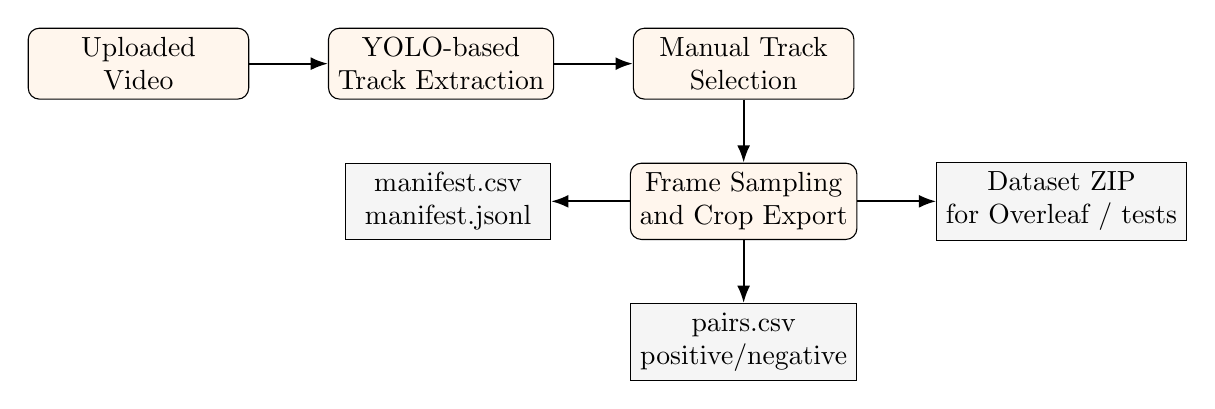
\begin{tikzpicture}[
  node distance=0.8cm and 1cm,
  box/.style={draw, rounded corners, align=center, minimum width=2.8cm, minimum height=0.9cm, fill=orange!7},
  file/.style={draw, align=center, minimum width=2.6cm, minimum height=0.8cm, fill=gray!8},
  arrow/.style={-{Latex[length=2.2mm]}, thick}
]
\node[box] (video) {Uploaded\\Video};
\node[box, right=of video] (tracks) {YOLO-based\\Track Extraction};
\node[box, right=of tracks] (select) {Manual Track\\Selection};
\node[box, below=of select] (sample) {Frame Sampling\\and Crop Export};
\node[file, left=of sample] (manifest) {manifest.csv\\manifest.jsonl};
\node[file, below=of sample] (pairs) {pairs.csv\\positive/negative};
\node[file, right=of sample] (zip) {Dataset ZIP\\for Overleaf / tests};

\draw[arrow] (video) -- (tracks);
\draw[arrow] (tracks) -- (select);
\draw[arrow] (select) -- (sample);
\draw[arrow] (sample) -- (manifest);
\draw[arrow] (sample) -- (pairs);
\draw[arrow] (sample) -- (zip);
\end{tikzpicture}

  \caption{GUI-supported video-to-testset workflow. The exported dataset is designed for later evaluation scripts and manual inspection.}
  \label{fig:dataset-pipeline}
\end{figure}

\section{Software Structure}

The codebase has been reorganized around a Python package and clear project-level directories. The core package contains configuration loading, application orchestration, CLI logic, algorithm modules, storage wrappers, and dataset export helpers. Applications such as the Streamlit GUI live in \texttt{apps/}; research scripts live in \texttt{experiments/}; generated datasets and runtime databases are excluded from version control by default.

\begin{table}[htbp]
  \centering
  \caption{Current repository organization relevant to the dissertation artifact.}
  \label{tab:repo-structure}
  \begin{tabularx}{\textwidth}{lX}
    \toprule
    Directory & Responsibility \\
    \midrule
    \texttt{crossmedia\_pid/} & Importable package: configuration, pipeline orchestration, core modules, storage, dataset export. \\
    \texttt{apps/} & Streamlit GUI entry points. \\
    \texttt{experiments/} & Evaluation and exploratory scripts. \\
    \texttt{experiments/generated\_datasets/} & GUI-exported crop datasets, ignored by version control. \\
    \texttt{configs/} & Local configuration and shareable example configuration. \\
    \texttt{docs/dissertation/} & Overleaf-compatible multi-paper dissertation draft. \\
    \bottomrule
  \end{tabularx}
\end{table}

\section{Evaluation Metrics}

The final dissertation evaluation will use pair-level and retrieval-level metrics. Pair-level evaluation treats each crop pair as a binary same-person or different-person decision. For a threshold $\tau$, a pair is predicted positive if its score is at least $\tau$. Precision, recall, and F1 are defined in the standard way:

\begin{equation}
\mathrm{Precision} = \frac{TP}{TP + FP}, \quad
\mathrm{Recall} = \frac{TP}{TP + FN}, \quad
\mathrm{F1} = \frac{2PR}{P + R}.
\end{equation}

Retrieval-level evaluation will use top-$k$ accuracy and mean average precision where a gallery is available. The GUI-generated \texttt{pairs.csv} file supports pair-level analysis immediately, while the \texttt{manifest.csv} file supports later conversion into query/gallery retrieval splits.

\section{Experimental Design}

The dissertation will distinguish three experiment types. First, \textbf{component ablations} compare dense-only, sparse-only, and hybrid scores. Second, \textbf{workflow experiments} evaluate whether GUI-generated datasets produce consistent labels and useful failure analysis metadata. Third, \textbf{cross-media extension experiments} test whether text descriptions can retrieve the correct person crops. This staged design avoids relying on a single headline score and instead evaluates the system as both a matching method and a research artifact.


\part{Paper-Based Manuscripts}
\chapter[Paper I: Hybrid VLM-Based Person Identification]{Paper I: Hybrid Vision--Language Attribute Representation for Cross-Media Person Identification}
\label{paper:hybrid-vlm-pid}

\section*{Manuscript Status}
\addcontentsline{toc}{section}{Manuscript Status}

This paper is a first full dissertation manuscript draft. It is based on the implemented \systemname\ prototype and will later be revised into a standalone conference-style paper after the evaluation dataset is expanded.

\section{Abstract}

Cross-media person identification requires matching individuals across still images, video frames, and potentially natural-language descriptions. Existing person re-identification systems often rely on dense visual embeddings that can be effective but difficult to inspect. This paper presents \systemname, a modular prototype that uses a vision--language model to extract structured person attributes and combines dense semantic embeddings with sparse attribute vectors for identity matching. The system uses YOLO-based person detection, VLM-based attribute extraction, a dynamic attribute registry, ChromaDB vector retrieval, and a threshold-based hybrid matcher. Preliminary controlled experiments indicate stable same-person matching across image pairs and video-frame crops, suggesting that attribute-grounded hybrid representations can support interpretable cross-media retrieval. The paper discusses the method, implementation, early findings, and limitations that motivate larger-scale evaluation.

\section{Introduction}

Person Re-ID has traditionally been formulated as an image retrieval problem: given a query person image, retrieve images of the same identity from a gallery \citep{zheng2016person,ye2021deep}. In practical settings, however, the query may not always be an image from the same distribution as the gallery. A user may begin with a short clip, a partial crop, or a description of clothing. This motivates representations that can be connected to both visual similarity and language-level attributes.

Vision--language models provide an opportunity to convert person crops into structured descriptions. Instead of relying solely on a black-box visual embedding, \systemname\ asks a VLM to produce a JSON-style set of attributes. These attributes are then used in two ways: as text for dense semantic embedding, and as symbolic keys for sparse vector matching. The central hypothesis is that dense and sparse evidence are complementary. Dense embeddings tolerate paraphrase and semantic similarity; sparse vectors preserve explicit overlap in detected traits.

This paper focuses on the first part of the dissertation: whether such a hybrid representation can be implemented as a coherent person identification pipeline. The paper does not claim that the current prototype exceeds state-of-the-art Re-ID systems. Instead, it positions \systemname\ as an interpretable research framework that can later be evaluated against stronger baselines such as strong CNN baselines, transformer-based Re-ID models, and CLIP-based Re-ID methods \citep{luo2019bag,he2021transreid,li2023clipreid}.

\section{Related Work}

\subsection{Image-Based Re-ID}

Image-based Re-ID benchmarks such as CUHK03 and Market-1501 provide the conventional setting for matching pedestrian images across cameras \citep{li2014deepreid,zheng2015scalable}. Strong Re-ID baselines combine classification and metric learning objectives, data augmentation, re-ranking, and carefully tuned training recipes \citep{luo2019bag}. Transformer approaches such as TransReID further improve representation learning by modelling global context and part-level cues \citep{he2021transreid}. These methods provide important baselines for future comparison, but their learned embeddings are not always easy to interpret.

\subsection{Attribute and Language Supervision}

Attribute-based methods use semantic cues to assist person retrieval. Deep attribute-driven Re-ID shows that attributes can provide complementary supervision for identity matching \citep{su2016deep}. Text-based person search, especially the CUHK-PEDES benchmark, further demonstrates the value of connecting person images with natural-language descriptions \citep{li2017personsearch}. \systemname\ borrows this semantic motivation but obtains descriptions automatically from VLMs instead of relying on human-written captions.

\subsection{Vision--Language Models for Re-ID}

Large-scale image--text pretraining has made visual representations more transferable \citep{radford2021learning}. CLIP-ReID adapts CLIP to person Re-ID by exploiting vision--language pretraining for image re-identification \citep{li2023clipreid}. The approach in this paper is complementary: rather than using a VLM only as a representation backbone, it uses the VLM to produce structured attributes that can be displayed, stored, and combined with sparse evidence.

\section{Method}

\subsection{Person Crop Extraction}

Given an image or sampled video frame, the visual extractor detects person bounding boxes and filters them by confidence and size. A crop quality score is computed from four factors: detection confidence, relative area, local sharpness, and centrality. For single-image processing, only the best crop is passed to the VLM. For video processing, crops may also be associated into trajectories.

Let $b=(x_1,y_1,x_2,y_2)$ denote a detected bounding box and $I_b$ its crop. The prototype quality score is not intended to be a learned perceptual measure; it is a pragmatic heuristic for selecting a crop that is large enough, sufficiently sharp, and likely to contain the main person. This simple heuristic is useful because the VLM stage is comparatively expensive, so passing every detection to the VLM would slow down exploratory testing.

\subsection{Structured Attribute Extraction}

The VLM prompt requests a fixed but open-ended set of appearance attributes. The target schema includes demographic cues, clothing colour and type, pattern type and description, accessories, hair, posture, and distinctive traits. The parser standardizes snake-case keys and removes unavailable values. Because VLM responses may not always be valid JSON, the implementation attempts direct parsing, code-block extraction, JSON repair, and brace-delimited fallback extraction.

The prompt design reflects a surveillance-style visual description task. In particular, it asks the model to describe pattern location, size, and colour when visible. This detail is important because two people may share the same broad clothing category but differ in a logo or printed pattern. The extracted attributes are stored together with the raw model response so that later failure analysis can distinguish between VLM extraction errors and matching errors.

\subsection{Dense Semantic Representation}

Attributes are linearized into a compact textual description such as \texttt{topwear\_color is black, shoes\_type is sneakers}. This text is encoded using a sentence embedding model. The dense vector is designed to capture semantic similarity even when attribute values are not identical strings.

\subsection{Sparse Attribute Representation}

Each observed attribute key is registered in a persistent attribute registry. The sparse representation is a dictionary from registry IDs to weights. The current prototype uses equal weights, but the design allows later weighting by reliability, attribute category, or empirical discriminativeness. The registry grows as new attributes appear, which avoids requiring a closed schema at the beginning of development.

\subsection{Hybrid Matching}

Candidate records are retrieved from ChromaDB using dense vector similarity. For each candidate, sparse similarity is computed using a weighted Jaccard-style overlap. The final score is a weighted sum of dense and sparse scores. A configurable threshold determines whether the query is assigned to an existing identity or creates a new identity.

The matching procedure can be summarized as follows. Given a query crop, extract attributes $A_q$, generate dense vector $d_q$ and sparse vector $s_q$, retrieve top-$k$ candidates by $d_q$, compute sparse overlap with each candidate, and choose the candidate with the highest hybrid score. If no candidate exceeds the threshold, the query is stored as a new identity. This design supports incremental database construction, which is useful for exploratory video analysis where identities are added over time.

\section{Implementation}

The implementation is organized as a Python package. The main application service is responsible for wiring together the extractor, VLM client, vectorizer, matcher, and storage layer. A CLI provides image processing and search commands, while the Streamlit GUI supports video-oriented workflows. Configuration is stored in YAML and API keys are read from environment variables.

The implementation also separates research scripts from production-like package code. Experimental scripts are kept under \texttt{experiments/}, while reusable logic such as configuration loading, application orchestration, and dataset export is in \texttt{crossmedia\_pid/}. This separation matters for dissertation reproducibility because it allows the text to describe a stable artifact rather than a collection of one-off scripts.

\begin{table}[htbp]
  \centering
  \caption{Core modules in the current implementation.}
  \label{tab:paper1-modules}
  \begin{tabularx}{\textwidth}{lX}
    \toprule
    Module & Role \\
    \midrule
    \texttt{PersonExtractor} & Detects and crops person regions from images or frames. \\
    \texttt{FeatureExtractor} & Calls a VLM provider and parses structured attributes. \\
    \texttt{DynamicVectorizer} & Generates dense text embeddings and sparse registry vectors. \\
    \texttt{IdentityMatcher} & Computes hybrid scores and assigns identity decisions. \\
    \texttt{ChromaStore} & Persists vectors and metadata for retrieval. \\
    \bottomrule
  \end{tabularx}
\end{table}

\section{Preliminary Results}

Early tests used paired person images and video frame crops. In controlled same-person comparisons, the system produced high match scores and consistent identity decisions across repeated runs. The performance monitor showed that VLM feature extraction dominates runtime, while detection, vector search, and matching are comparatively fast. These results are promising but should be treated as preliminary because the dataset remains small and controlled.

\begin{table}[htbp]
  \centering
  \caption{Preliminary performance profile from the prototype stage. Values are indicative and will be replaced by final experiments.}
  \label{tab:paper1-performance}
  \begin{tabular}{lrr}
    \toprule
    Stage & Approx. Time & Notes \\
    \midrule
    Image loading & $<0.01$s & Local file read. \\
    Person detection & $\sim0.3$s & YOLO inference on sample images. \\
    VLM attribute extraction & $3$--$10$s & Depends on API latency and model. \\
    Vectorization & $\sim2$s & Includes embedding model call. \\
    Database matching & $<0.01$s & Small ChromaDB collection. \\
    \bottomrule
  \end{tabular}
\end{table}

\section{Planned Ablations}

The final version of this paper will include four ablation settings:

\begin{enumerate}
  \item \textbf{Dense only:} use only semantic embedding similarity.
  \item \textbf{Sparse only:} use only attribute-registry overlap.
  \item \textbf{Hybrid fixed weights:} use the current manually configured dense/sparse weights.
  \item \textbf{Hybrid tuned weights:} select weights and threshold on a validation split.
\end{enumerate}

These ablations will test whether sparse attribute evidence contributes beyond dense semantic embeddings. The expected result is not that sparse vectors always outperform dense vectors, but that they improve interpretability and help in cases where explicit traits such as bags, hats, or logos are visible.

\section{Discussion}

The hybrid representation offers two practical advantages. First, it creates an interpretable audit trail: the system can display extracted attributes alongside match scores. Second, it provides a path to text-based search, because natural-language descriptions and VLM-derived attributes can be mapped into the same representation space. The main weakness is that VLM attributes can vary with crop quality, viewpoint, and prompt design. A person whose logo or accessory is occluded may receive a substantially different sparse representation across frames.

Another challenge is that attributes are not equally discriminative. ``Black top'' may be common in a dataset, whereas ``red backpack'' may be more useful. A future learned weighting scheme could estimate attribute reliability and discriminativeness from the generated datasets. Until such data is available, the current implementation keeps the sparse representation deliberately simple.

\section{Limitations and Next Steps}

The current evaluation is not yet sufficient for final claims about accuracy. The next stage must construct a larger labelled dataset, compare against visual embedding baselines, conduct threshold sensitivity analysis, and measure false positives under visually similar clothing. Face embeddings are reserved as a future optional component, but the core dissertation contribution remains the attribute-grounded hybrid representation.

\section{Threats to Validity}

There are four main threats to validity. First, small pilot datasets may overestimate performance because they do not contain enough visually similar distractors. Second, VLM APIs may change over time, which can affect reproducibility. Third, the same-person labels generated from manual track selection are only as reliable as the underlying track quality. Fourth, the current sparse vector design uses attribute keys rather than full key--value facts, which may understate the discriminative value of attributes. These threats motivate the dataset creation workflow in Paper II and the registry protocol in Paper III.

\section{Conclusion}

This paper introduced \systemname\ as a modular method for cross-media person identification. The prototype demonstrates that VLM-derived attributes can be converted into a hybrid representation suitable for interpretable matching. The method is not a replacement for mature Re-ID models; rather, it is a research framework for combining semantic attributes, vector retrieval, and human-readable evidence in cross-media workflows.

\chapter[Paper II: GUI-Assisted Video Testset Creation]{Paper II: GUI-Assisted Video Testset Creation for Cross-Media Person Identification}
\label{paper:video-testset-gui}

\section*{Manuscript Status}
\addcontentsline{toc}{section}{Manuscript Status}

This paper is a working draft based on the newly implemented Streamlit GUI and dataset export module. The experimental section is currently scaffolded; final results will be added after larger video samples are annotated.

\section{Abstract}

Evaluation is a bottleneck for early-stage cross-media person identification systems because labelled same-person and different-person pairs are costly to create. This paper presents a GUI-assisted workflow for constructing test datasets from video. The system uploads a video, detects and tracks person trajectories, allows the researcher to select candidate identities, samples frames from selected tracks, exports cropped person images, and generates a manifest plus positive and negative pair files. The workflow is implemented in the \systemname\ Streamlit interface and produces Overleaf- and script-friendly dataset artifacts. By turning exploratory video analysis into structured testset creation, the interface supports iterative evaluation, manual inspection, and future benchmark expansion.

\section{Motivation}

The first prototype of \systemname\ could process individual images and compare selected frames, but evaluation still required manual file handling. For a dissertation project with limited time, this creates friction: every new video requires repeated manual extraction, naming, and pair construction. A GUI-supported dataset workflow reduces this overhead and encourages more systematic experiments.

This paper treats the GUI as part of the research method rather than as a presentation layer only. The interface determines how data is selected, how crops are produced, what metadata is saved, and how easily failure cases can be revisited. A poorly designed interface can quietly bias evaluation by encouraging cherry-picked samples or by losing track of source-frame context. The current design therefore emphasizes explicit track selection, visible quality metadata, and exportable manifests.

\section{Design Requirements}

The GUI was designed around five requirements:

\begin{enumerate}
  \item \textbf{Low friction.} A researcher should be able to upload a video and create a dataset without writing one-off extraction scripts.
  \item \textbf{Human-in-the-loop labelling.} The interface should keep the researcher responsible for selecting tracks instead of assuming perfect automatic identity tracking.
  \item \textbf{Traceability.} Every exported crop should retain its source video, frame number, track ID, and bounding-box coordinates.
  \item \textbf{Script compatibility.} The output should be usable by Python evaluation scripts without requiring the GUI.
  \item \textbf{Overleaf compatibility.} Crops and summaries should be easy to inspect and include in dissertation figures or appendices.
\end{enumerate}

\section{Workflow Design}

The GUI workflow has five stages:

\begin{enumerate}
  \item Upload a video file in a common format such as MP4, AVI, MOV, or MKV.
  \item Sample frames and detect person bounding boxes using the visual extractor.
  \item Associate detections into lightweight tracks using bounding-box overlap.
  \item Display track previews, frame counts, position distributions, and quality scores.
  \item Export selected tracks as a labelled crop dataset.
\end{enumerate}

The interface intentionally keeps manual selection in the loop. Fully automatic identity labelling would be unreliable at the current stage, especially when multiple people overlap or when tracking fragments occur. Manual track selection lets the researcher choose identities that are suitable for controlled testing while still automating the repetitive export steps.

The GUI also provides a quick same-person test for a selected track. It extracts two crops from different positions when possible, processes them through \systemname, and displays the identity decision, match score, quality score, and extracted attributes. This immediate feedback helps the researcher decide whether a video is useful for building a larger testset.

\section{Dataset Format}

The exported dataset contains a simple directory structure:

\begin{lstlisting}
dataset_name/
  images/
    p0000_track000_f000015_left_00.jpg
    p0000_track000_f000120_right_01.jpg
  manifest.csv
  manifest.jsonl
  pairs.csv
  summary.json
\end{lstlisting}

\texttt{manifest.csv} records one row per crop, including the relative image path, assigned person ID, source track ID, frame number, position label, detection confidence, track statistics, bounding box coordinates, and source video path. \texttt{pairs.csv} contains positive pairs from crops of the same selected track and negative pairs from crops of different selected tracks. \texttt{summary.json} records dataset-level metadata such as identity count, image count, and pair counts.

\begin{table}[htbp]
  \centering
  \caption{Key fields in the generated manifest.}
  \label{tab:manifest-fields}
  \begin{tabularx}{\textwidth}{lX}
    \toprule
    Field & Meaning \\
    \midrule
    \texttt{image\_path} & Relative path to the exported crop. \\
    \texttt{person\_id} & Dataset-local identity label assigned from selected track order. \\
    \texttt{track\_id} & Original GUI track identifier. \\
    \texttt{frame\_number} & Video frame from which the crop was extracted. \\
    \texttt{position} & Coarse horizontal position: left, center, right, or unknown. \\
    \texttt{confidence} & Detector confidence for the sampled frame. \\
    \texttt{bbox\_*} & Padded crop coordinates in the source frame. \\
    \bottomrule
  \end{tabularx}
\end{table}

\section{Implementation}

The export logic is implemented separately from the Streamlit page in \texttt{crossmedia\_pid/dataset.py}. This separation prevents the GUI from becoming the only way to generate datasets and makes the export function testable. A lightweight unit test creates a synthetic video, exports crops from two mock tracks, and checks that images, manifests, pairs, and ZIP archives are generated correctly.

The export function samples each selected track at approximately evenly spaced indices. This avoids taking all crops from adjacent frames, which would make same-person pairs too easy and uninformative. For each sampled frame, the function expands the bounding box by a configurable padding factor and saves a JPEG crop. Positive pairs are generated from combinations of crops within the same selected track. Negative pairs are generated across selected tracks. The current negative-pair strategy is intentionally simple and will be refined once larger videos are available.

\section{Quality Control}

The exported manifest enables several quality checks before running expensive VLM evaluation:

\begin{itemize}
  \item remove tracks with fewer than a minimum number of sampled frames;
  \item inspect crops with low detector confidence;
  \item compare failures by horizontal position to detect viewpoint sensitivity;
  \item trace any crop back to its source frame and bounding box;
  \item verify that positive pairs are not merely near-duplicate adjacent frames.
\end{itemize}

These checks are important because dataset errors would directly distort the evaluation of the matching algorithm. For example, a fragmented track may create false positive labels if it merges two individuals, while an identity split may create false negative pairs if the same person is selected as two different tracks.

\section{Preliminary Evaluation Plan}

The exported datasets will support three levels of evaluation:

\begin{itemize}
  \item \textbf{Pair-level matching.} Each positive or negative pair can be processed by \systemname\ to compute similarity scores and binary decisions.
  \item \textbf{Threshold sensitivity.} The same pairs can be evaluated under different match thresholds to estimate precision--recall trade-offs.
  \item \textbf{Failure analysis.} Manifest metadata allows failure cases to be grouped by position, track quality, frame number, and crop confidence.
\end{itemize}

The final dissertation experiments should include at least three categories of videos: single-person controlled movement, multi-person non-overlapping scenes, and multi-person scenes with visual similarity or occlusion. The current text reports the planned structure; final dataset statistics and measured results should be inserted after annotation is complete.

\begin{table}[htbp]
  \centering
  \caption{Planned dataset categories for GUI-generated evaluation.}
  \label{tab:paper2-dataset-plan}
  \begin{tabularx}{\textwidth}{lX}
    \toprule
    Category & Purpose \\
    \midrule
    Single-person controlled videos & Verify same-person consistency across pose and position changes. \\
    Multi-person separated videos & Generate simple positive and negative pairs with low tracking ambiguity. \\
    Multi-person similar-clothing videos & Stress-test false positives and attribute ambiguity. \\
    Occlusion or low-resolution clips & Analyse failure cases under difficult visual evidence. \\
    \bottomrule
  \end{tabularx}
\end{table}

\section{Discussion}

The dataset creation interface is not merely an engineering convenience. It changes the research workflow by making evaluation iterative. When a matching error occurs, the researcher can inspect the source crop, track position, VLM attributes, and pair label. This is especially important for a VLM-based system because errors may arise from detection quality, crop context, prompt instability, or database thresholding.

The workflow also supports dissertation writing. Exported crops can be used as qualitative examples, \texttt{summary.json} provides dataset statistics, and \texttt{pairs.csv} can be used to regenerate evaluation tables. This makes the GUI a bridge between software development and thesis evidence.

\section{Limitations}

The current workflow does not solve identity tracking in complex scenes. It uses a lightweight IoU-based association strategy, so it can fail under long occlusions, camera cuts, or crossing pedestrians. It also assumes that the researcher can manually identify usable tracks. These limitations are acceptable for the present dissertation stage because the goal is controlled dataset construction, not fully automatic multi-camera tracking.

\section{Conclusion}

This paper presented a GUI-assisted video-to-testset workflow for \systemname. The workflow converts videos into structured crop datasets with manifests and labelled pairs, creating a foundation for the dissertation's final evaluation. The current implementation is ready for pilot data creation and will be extended with larger annotated experiments.

\chapter[Paper III: Dynamic Attribute Registry and Evaluation Protocol]{Paper III: Dynamic Attribute Registry and Evaluation Protocol for Attribute-Grounded Person Retrieval}
\label{paper:attribute-registry-protocol}

\section*{Manuscript Status}
\addcontentsline{toc}{section}{Manuscript Status}

This chapter is a manuscript-in-preparation. It currently defines the conceptual direction for the third paper and will be expanded after the final dataset and ablation experiments are complete.

\section{Abstract}

Vision--language models can produce flexible descriptions, but open-ended attributes create a representation challenge: the system must support new attribute keys without constantly redesigning its vector schema. This paper proposes a dynamic attribute registry for attribute-grounded person retrieval. The registry maps observed attribute keys to persistent sparse dimensions and tracks usage statistics over time. The paper further proposes an evaluation protocol for measuring the contribution of dense semantic similarity, sparse attribute overlap, and future text-query alignment. The protocol will guide the final stage of \systemname\ evaluation.

\section{Motivation}

A closed attribute schema is easy to evaluate but restrictive. A fully open text description is flexible but difficult to index and compare. \systemname\ currently takes a middle path: it asks the VLM for a target set of attributes, but the sparse representation can grow when new keys appear. This supports experimentation with new prompts and attribute categories without invalidating previously stored dense vectors.

The problem is especially visible in person retrieval because some cues are stable categories, such as \texttt{topwear\_color}, while others are open-ended, such as the description of a printed logo. A rigid schema may miss useful details, but a completely unconstrained set of generated phrases may make sparse matching meaningless. The dynamic registry is therefore a compromise between controlled vocabulary and open-world description.

\section{Dynamic Attribute Registry}

The registry stores a mapping from normalized attribute keys to integer identifiers. Each key also records observation count and timestamps. In the current implementation, the sparse vector records key presence rather than value-specific dimensions. This design is intentionally simple; it avoids uncontrolled explosion from every possible colour or phrase, while still measuring whether two descriptions contain overlapping categories of evidence.

The registry currently supports three operations. First, \textbf{registration} assigns a new identifier when an unseen normalized key appears. Second, \textbf{lookup} retrieves the identifier for a known key. Third, \textbf{statistics} reports the number of observed and frequently observed attributes. These operations are sufficient for the prototype, but the dissertation evaluation will use the registry statistics to identify which attributes are common, rare, stable, or noisy.

Future versions should consider three extensions:

\begin{enumerate}
  \item \textbf{Value-aware dimensions:} represent pairs such as \texttt{topwear\_color=black} instead of only \texttt{topwear\_color}.
  \item \textbf{Reliability weights:} down-weight attributes that are frequently unstable across frames.
  \item \textbf{Category priors:} assign higher weights to more discriminative categories such as logos, bags, or unusual clothing patterns.
\end{enumerate}

\section{Proposed Weighting Strategy}

A natural extension is to replace equal sparse weights with reliability-aware weights. Let $a$ be an attribute key and let $r(a)$ denote its empirical repeatability across crops of the same identity. Let $u(a)$ denote its uniqueness across identities. A future sparse weight could be defined as:

\begin{equation}
w(a) = \lambda r(a) + (1-\lambda)u(a),
\end{equation}

\noindent where $\lambda$ controls the trade-off between stability and discriminativeness. For example, a very common attribute such as \texttt{topwear\_type} may be stable but not unique, while a logo description may be unique but less reliably extracted. The final dissertation may not fully implement this weighting scheme, but it provides a principled direction for future work.

\section{Evaluation Protocol}

The final evaluation should report:

\begin{itemize}
  \item accuracy, precision, recall, F1, and ROC/AUC for pair-level matching;
  \item separate dense-only, sparse-only, and hybrid matching ablations;
  \item threshold sensitivity curves for the final identity decision;
  \item stability of VLM attributes across frames of the same track;
  \item qualitative failure cases grouped by occlusion, low resolution, similar clothing, and attribute hallucination.
\end{itemize}

The protocol should be applied first to GUI-generated crop datasets and then, if time permits, to public Re-ID or text-based person search datasets. Public datasets such as Market-1501 and CUHK-PEDES are useful because they allow comparison to established tasks, but the dissertation's own generated datasets remain important because they reflect the actual workflow supported by the software artifact.

\section{Text-to-Person Extension}

The registry also prepares the system for text-to-person retrieval. A user description can be parsed into attributes, vectorized using the same dense and sparse pathways, and searched against the existing database. This would transform \systemname\ from an image/video matching prototype into a cross-media retrieval tool. The main research question is whether VLM-derived attributes and human-written descriptions are aligned enough to share a representation space.

Text-to-person retrieval can be implemented in two stages. In the first stage, a deterministic parser or language model converts a text query into the same attribute keys used by VLM extraction. In the second stage, the query attributes are vectorized and searched against stored person records. This design is inspired by natural-language person search research \citep{li2017personsearch}, but it differs because the database entries are generated by VLM descriptions rather than human captions.

\section{Planned Experiments}

\begin{table}[htbp]
  \centering
  \caption{Planned ablation experiments for Paper III.}
  \label{tab:paper3-planned-experiments}
  \begin{tabularx}{\textwidth}{lX}
    \toprule
    Experiment & Purpose \\
    \midrule
    Dense-only retrieval & Measure baseline semantic embedding performance. \\
    Sparse-only retrieval & Measure effect of explicit attribute overlap. \\
    Hybrid retrieval & Test whether dense and sparse evidence are complementary. \\
    Prompt variants & Measure sensitivity to VLM extraction prompt wording. \\
    Text queries & Evaluate whether natural descriptions retrieve correct video crops. \\
    \bottomrule
  \end{tabularx}
\end{table}

\section{Expected Outcomes}

The expected outcome is a clearer understanding of when attribute-grounded retrieval helps. Dense-only retrieval is expected to be more tolerant of paraphrase and minor wording differences. Sparse-only retrieval is expected to be more interpretable but less robust when attributes are missing. Hybrid retrieval should perform best when dense semantics and explicit attribute overlap agree. Text-query retrieval is expected to be more difficult than image-pair matching because user descriptions may omit details that the VLM includes or include details that the VLM fails to detect.

\section{Risks}

The main risk is that the registry grows in ways that are not semantically meaningful. If the VLM produces inconsistent keys, the sparse space becomes noisy. This risk is partly addressed by key normalization and prompt control, but future work may require synonym mapping or ontology-based grouping. Another risk is that value-aware dimensions will create too many sparse features. The dissertation should therefore evaluate the simplest registry first before adding complexity.

\section{Conclusion}

This manuscript will turn the current engineering mechanism of a dynamic registry into a formal research contribution. Its role in the dissertation is to connect the implemented prototype to a broader question: how should open-ended VLM attributes be stabilized, indexed, and evaluated for person retrieval?


\part{Synthesis}
\chapter{Integrative Discussion}
\label{ch:integrative-discussion}

\section{What the Papers Share}

The three manuscripts are connected by a single theme: cross-media person identification should be both vector-searchable and inspectable. Paper I introduces the hybrid representation, Paper II creates the evaluation workflow needed to study it, and Paper III frames the dynamic attribute registry as the mechanism that can make open-ended VLM descriptions usable at scale.

\section{Strengths of the Current Prototype}

The current prototype has several strengths. It is modular, which makes it possible to replace the VLM provider, embedding model, vector database, or matching weights without rewriting the entire system. It is also operational: the CLI and GUI can process images and videos, and the GUI can now export reusable datasets. Finally, the system produces human-readable attributes, which helps diagnose why a match succeeded or failed.

\section{Current Limitations}

The limitations are equally important. The evaluation dataset remains small, and the reported performance should be treated as preliminary. The VLM may produce unstable descriptions across frames, especially when crops are blurry, occluded, or low resolution. The current sparse vector records attribute keys rather than value-level facts, which limits its discriminative power. The tracking algorithm in the GUI is lightweight and can fragment identities in complex scenes. Finally, API-based VLM calls introduce latency, cost, and reproducibility concerns.

\section{Implications for Final Evaluation}

The final dissertation should avoid overclaiming. The strongest defensible claim is not that \systemname\ outperforms mature Re-ID models, but that it provides an interpretable and extensible framework for VLM-assisted cross-media person matching. The final evaluation should therefore include both quantitative matching metrics and qualitative interpretability analysis. Failure cases should be treated as evidence, not merely as errors to hide.

\section{Ethical and Practical Considerations}

Person identification technologies raise privacy and misuse concerns. This dissertation should explicitly frame \systemname\ as a research prototype and avoid presenting it as a deployment-ready surveillance system. Any dataset collection should respect consent, data minimization, and local institutional guidelines. The dissertation should also discuss bias risks: VLMs may describe demographic traits inconsistently, and clothing-based matching can be unreliable or socially sensitive. The most responsible use of this work is as a controlled research artifact for studying representation and evaluation, not as an automated decision system.

\chapter{Conclusion and Future Work}
\label{ch:conclusion}

\section{Summary}

This dissertation develops \systemname, a modular prototype for cross-media person identification. The system uses visual detection to obtain person crops, VLM prompting to extract structured attributes, dense and sparse vectorization to represent those attributes, and a hybrid matcher to assign identity decisions. Recent engineering work reorganized the codebase into a maintainable package structure and added a GUI-based video testset creation workflow.

\section{Contributions}

The current dissertation draft contributes:

\begin{enumerate}
  \item a working VLM-assisted person identification pipeline;
  \item a hybrid dense--sparse representation for attribute-grounded matching;
  \item a dynamic registry for open-ended attribute dimensions;
  \item a GUI workflow for converting videos into labelled crop datasets;
  \item an Overleaf-compatible paper-based dissertation structure for continuing the writing process.
\end{enumerate}

\section{Future Work}

The immediate next step is to generate and annotate larger test datasets using the new GUI. After that, the dissertation should add final experiments, including dense-only and sparse-only ablations, threshold tuning, text-query retrieval, and failure-case analysis. A future system version may integrate face embeddings, stronger tracking, caching, and local VLM inference to reduce latency and improve reproducibility.

\section{Closing Remarks}

The project began as an implementation-heavy prototype and is now ready to become a dissertation argument. The central argument is that VLM-derived attributes can make person matching more interpretable and more adaptable to cross-media workflows, provided that the system is evaluated carefully and its limitations are made explicit.


\appendix
\chapter{Software Artifact}
\label{app:software}

\section{Repository Layout}

The software artifact is organized as a Python project. The main package is \texttt{crossmedia\_pid}. GUI entry points are kept in \texttt{apps/}; experiments are kept in \texttt{experiments/}; generated datasets are ignored by version control.

\section{Common Commands}

\begin{lstlisting}[language=bash]
conda activate crossmedia
python -m crossmedia_pid.cli process path/to/image.jpg
python -m crossmedia_pid.cli stats
streamlit run apps/video_test_webgui.py
python -m pytest tests/test_dataset_export.py
\end{lstlisting}

\section{Verification Completed}

At this draft stage, the Python files parse successfully, the CLI help command runs in the configured Conda environment, and the dataset export unit test passes. Full end-to-end VLM evaluation requires a valid API key and selected test videos.

\chapter{Configuration Example}
\label{app:configuration}

The project uses a YAML configuration file. Secrets are not stored in version control; API keys should be provided through environment variables.

\begin{lstlisting}[language=yaml]
models:
  yolo:
    model_path: "models/yolov8n.pt"
    conf_threshold: 0.5
    iou_threshold: 0.45

  vlm:
    provider: "aliyun"
    api_key: "${DASHSCOPE_API_KEY}"
    model_name: "qwen-vl-plus"
    max_tokens: 512
    temperature: 0.1

database:
  chroma:
    persist_directory: "data/chroma_db"
    collection_name: "person_embeddings"
    distance_fn: "cosine"

matching:
  threshold: 0.72
  top_k: 5
  weights:
    dense: 0.65
    sparse: 0.35
    face: 0.0
\end{lstlisting}


\backmatter
\bibliographystyle{plainnat}
\bibliography{references}

\end{document}
